\section{仿生机器鼠模型}
经过数十年的研究,现有的仿生机器鼠模型在尺寸和结构上已与生物鼠相近,且能够产生绝大数多数与生物鼠相似的交互行为,这为本文的研究提供了坚实的基础。我们设计并优化的仿生机器鼠(后称机器鼠模型,图\ref{figure_ratbot})具有优异的产生仿鼠运动的能力\cite{liDesignOptimizationLightweight2020},本文将利用这一模型开展研究。该模型的主要特点包括:
\begin{figure}[htbp]
  %\vspace{13pt}
  \centering
  \subfigure[机器鼠模型]{
  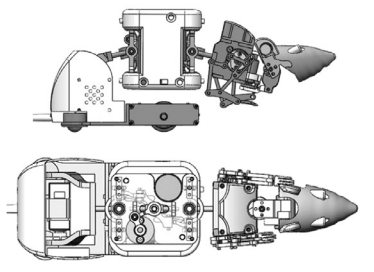
\includegraphics[width=0.45\linewidth]{images/ch02/ratbot.png} \label{figure_ratbot_model}
  }
  \subfigure[腰部机构]{
  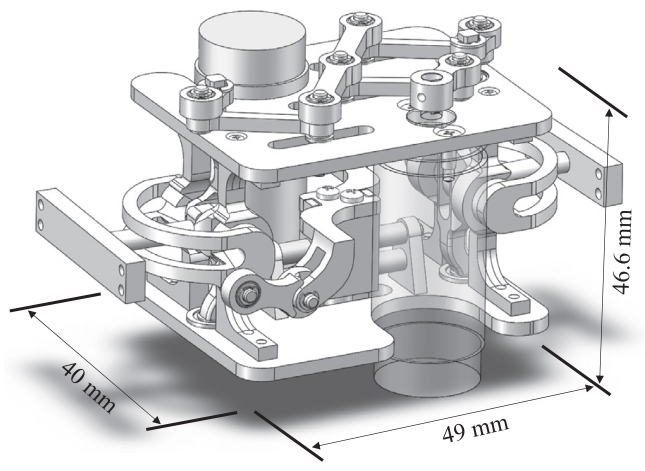
\includegraphics[width=0.45\linewidth]{images/ch02/compact-waist.png} \label{figure_ratbot_waist}
  }
  \caption{机器鼠模型及其腰部机构\cite{liDesignOptimizationLightweight2020}}\label{figure_ratbot} % label 用来在文中索引
\end{figure}
\begin{enumerate}[leftmargin=0em, topsep=0em, label=(\theenumi)]
%\setlength{\leftmargin}{0em}
\setlength{\itemindent}{4em}
\setlength{\labelsep}{0em}
\setlength{\labelwidth}{2em}
\setlength{\parsep}{0em}
\setlength{\itemsep}{0em}
\setlength{\topsep}{0em}
  \item 轮式驱动。
  \item 腰部灵活。
  \item 质量较小,运动灵活。
\end{enumerate}

此外,机器鼠模型躯干部分拥有7个主动自由度,其头颈部活动范围广,响应速度快,能够执行嗅探、探索等高频动作。是较为理想的开展行为交互实验的媒介。其部分关键属性与生物鼠比较如表\ref{table_spec}所示。
\begin{table}[htbp]
  \linespread{1.5}
  \zihao{5}
  \centering
  \caption{方式机器鼠关键属性}\label{table_spec}
  \begin{tabular}{*{3}{>{\centering\arraybackslash}m{1.5cm}}*{3}{>{\centering\arraybackslash}m{2.5cm}}}
    \toprule
    质量 & 体长 & 体宽 & 初始姿态高度    & 自由度数目 & 最大速度 \\ \midrule
    $400~g$&$195~mm$&$56~mm$&$74~mm$&$11$&$1.5~ms$\\
    \bottomrule
    \end{tabular}
\end{table}
